\documentclass{article}
\usepackage[utf8]{inputenc}
\usepackage{graphicx}
\graphicspath{ {./images/} }

\title{ECON 5253: PS6}
\author{William Lorton}
\date{March 18, 2021}

\usepackage{natbib}
\usepackage{graphicx}
\usepackage{hyperref}

\begin{document}

\maketitle

\section{Cleaning Data}

I'm building on the college football data frame that I made in the last problem set by adding in a new variable that indicates whether a given FBS team won the national title in a given year. This test example is used on data from the 2000 season and is therefore based upon the decision of the BCS in that year. I used the gsub() function to remove unwanted string information under the national championship winner variable and then used the ifelse() function to create a binary variable that indicates whether a given team won the national title (1 if so, 0 if not). I then added this vector of binary elements to the main df for the 2000 season.

\space 

The goal of course will be to have this national champion variable for every season that I want to look at. I could possibly write a loop for this, but there is likely a better way of going about it; I will think about it more later. One of the main challenges is the fact that there can be a different number of FBS teams in different seasons, which makes repetition of the national title winner team string for every row in the main data frame followed by a simple row-wise string comparison difficult.

\section{Visualizations}

Some miscellaneous visualizations of the FBS team records data I had on hand in my PS6 R script. These aren't really informative for my project, but the related code gives a framework for producing visualizations that I'd like to use in my paper. I've made bar plots for the average number of total wins per team by conference, the ten teams with the highest average number of home wins per season, and the ten teams with the highest average number of away wins per season from the 2000 season through the 2020 season.

\begin{figure}[h]
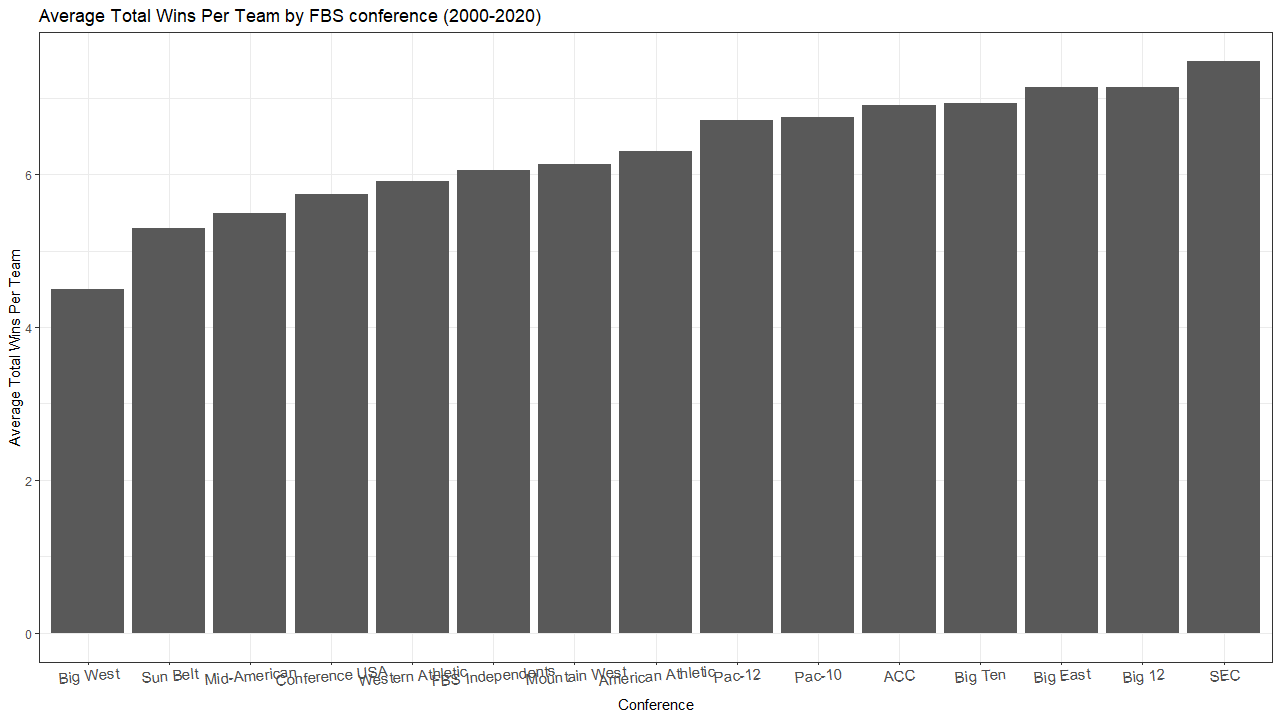
\includegraphics[width = 16cm, height = 11cm]{images/PS6a_Lorton.png}
\end{figure}

\begin{figure}[h]
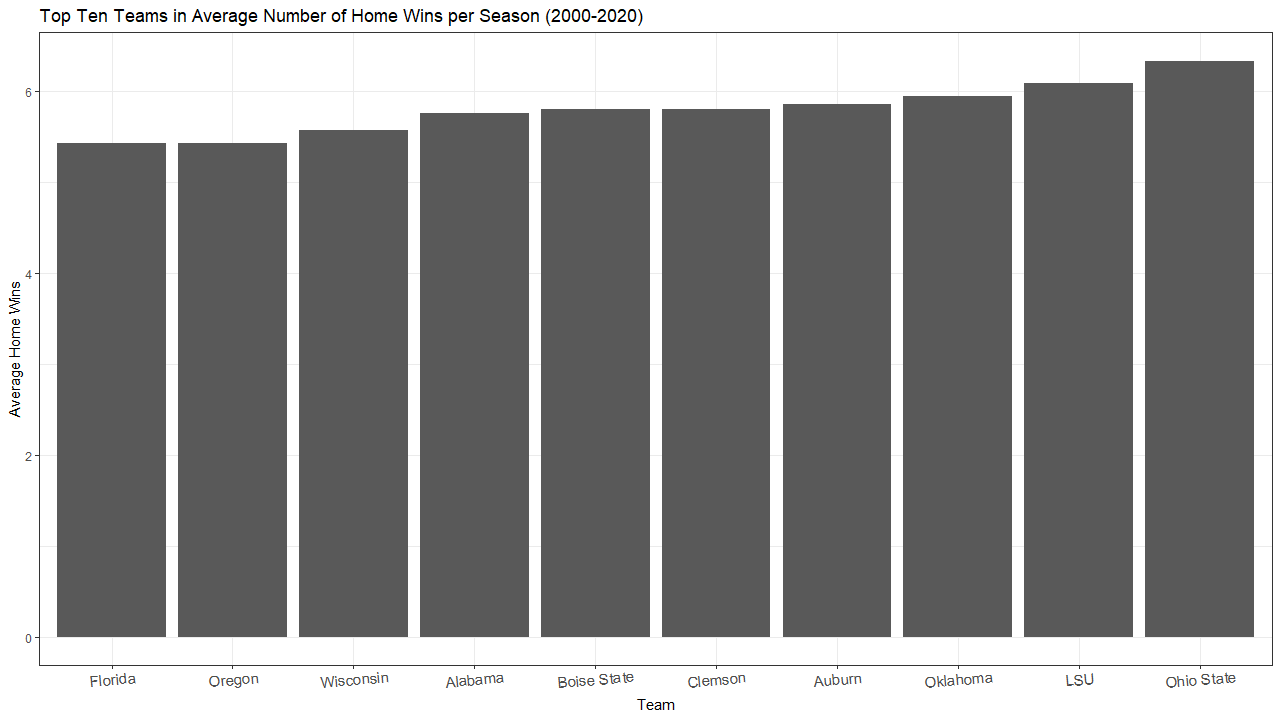
\includegraphics[width = 16cm, height = 11cm]{images/PS6b_Lorton.png}
\end{figure}

\begin{figure}[h]
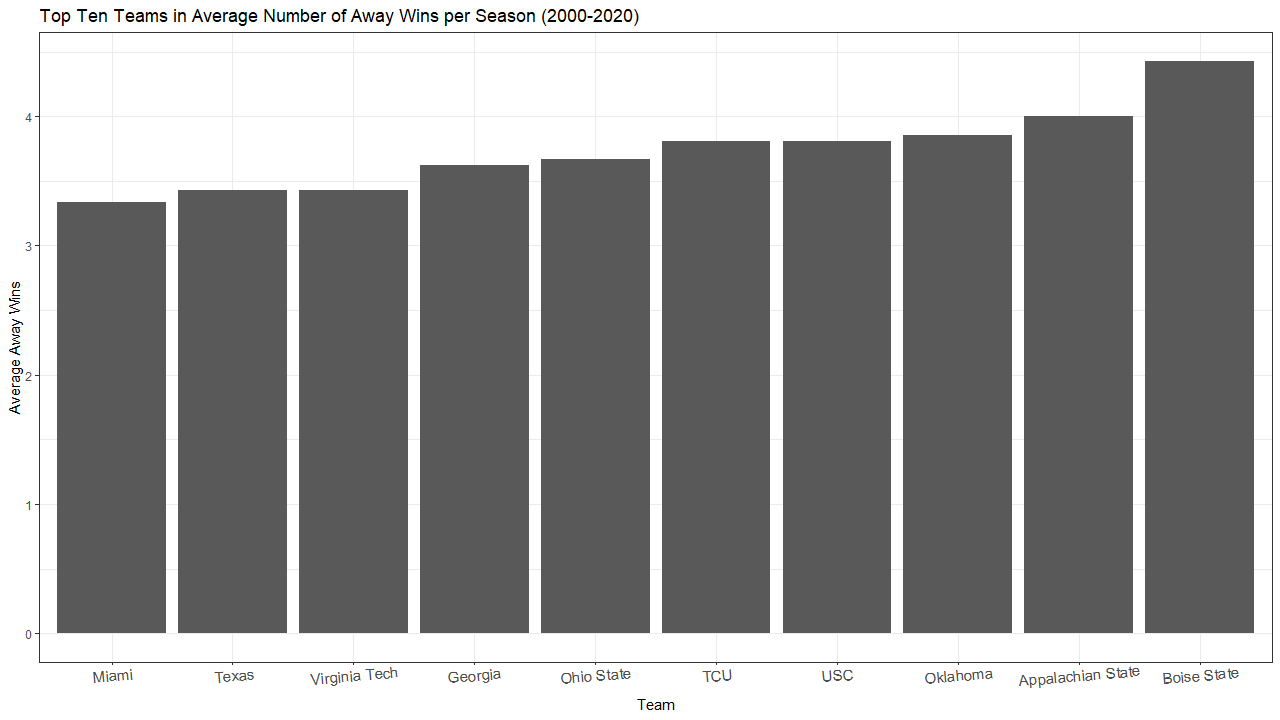
\includegraphics[width = 16cm, height = 11cm]{images/PS6c_Lorton.png}
\end{figure}


\end{document}
